%! Author = Nhan Huynh
%! Date = 10/01/2022

% Preamble
\documentclass{../tuda-beamer}
\usepackage{biblatex}


% Document
\begin{document}
    \maketitle

    \begin{frame}{Überblick}
        \tableofcontents
    \end{frame}


    \section{Fehlerbehandlung [20min]}
    \label{sec:fehlerbehandlung}
    \begin{frame}[c]{Fehlerbehandlung}
        \begin{figure}[h]
            \centering
            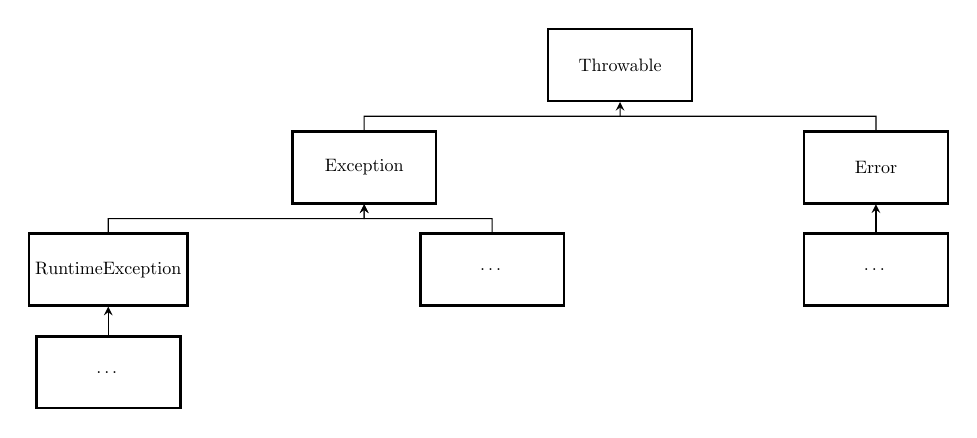
\begin{tikzpicture}[scale=.65, transform shape]
                \begin{scope}[
                    every node/.style={
                    draw,
                    line width=1pt,
                    minimum height=40pt,
                    minimum width=80pt,
                    transform shape,
                    shape=rectangle,
                    }
                ]
                    \node (a) at (0, 0) {Throwable};
                    \node (b) at (-5, -2) {Exception};
                    \node (c) at (5, -2) {Error};
                    \node (d) at (-10, -4) {RuntimeException};
                    \node (e) at (-10, -6) {\dots};
                    \node (f) at (-2.5, -4) {\dots};
                    \node (g) at (5, -4) {\dots};

                    \draw[-stealth] (0, -1) -- (a);
                    \draw (b.north) -- (-5, -1) -- (0, -1);
                    \draw (c.north) -- (5, -1) -- (0, -1);
                    \draw[-stealth] (d.north) -- (-10, -3) -- (-5, -3) -- (b.south);
                    \draw[-stealth] (e.north) -- (d.south);
                    \draw[-stealth] (f.north) -- (-2.5, -3) -- (-5, -3) -- (b.south);
                    \draw[-stealth] (g.north) -- (c.south);
                \end{scope}
            \end{tikzpicture}
            \caption{Java Exception Hierarchy}
            \label{fig:java-exception-hierarchy}
        \end{figure}
    \end{frame}

    \subsection{Throwable}
    \label{subsec:throwable}
    \begin{frame}{Throwable}
        \begin{itemize}
            \item Basisklasse für \inlinejava{Exception} und \inlinejava{Error}
            \item Bietet \inlinejava{try}-\inlinejava{catch} Konstrukt an, um Fehlerzustände
            zu behandeln
            \begin{itemize}
                \item Funktioniert für \inlinejava{Throwable} und alle direkt oder indirekt
                abgeleiteten Klssen von \inlinejava{Throwable}
            \end{itemize}
        \end{itemize}

        \lstinputlisting[style=Java, label={lst:try-catch-example}]{codes/try-catch_example.java}
    \end{frame}

    \subsection{Error}
    \label{subsec:error}
    \begin{frame}[c]{Error}
        \begin{itemize}
            \item Wird typischerweise vom Laufzeitsystem geworfen
            \item Fälle: Fehler welche nach menschlichen Ermessen so gewichtig ist, dass wohl keine
            sinvolle Fehlerbehandlung möglich ist, sondern der Programmabbruch die beste Lösung
            zu sein scheint.
            \item \inlinejava{Error}-Klassen müssen nicht mit
            \inlinejava{try}-\inlinejava{catch}-Block gefangen werden
            \item Formaler Aufbau (Werfen eines Errors):

            \begin{center}
                \inlinejava{throw new Errorklassenname(Parameter);}
            \end{center}
            \item Subklassennamen enden mit \inlinejava{Error}
        \end{itemize}
    \end{frame}

    \subsubsection{AssertionError}
    \label{subsubsec:assertion-error}
    \begin{frame}{AssertionError}
        \begin{itemize}
            \item Spezielle abgeleitete Error-Klasse
            \item Java bietet eine sehr bequeme Sonderform mit AssertionError umzugehen
            \item Schlüsselwort: \inlinejava{assert}
            \begin{itemize}
                \item Müssen aktiviert werden!
            \end{itemize}
            \item Formaler Aufbau:

            \lstinputlisting[style=Java, label={lst:assertion-error}]{codes/assertion_error.java}
        \end{itemize}
    \end{frame}

    \begin{frame}[c]{Beispiel}
        \lstinputlisting[
            style=Java,
            label={lst:assertion-error-example}
        ]{codes/assertion_error_example.java}
    \end{frame}

    \subsection{Exception}
    \label{subsec:exception}
    \begin{frame}[c]{Exception}
        \begin{itemize}
            \item \enquote{Checked Exception}
            \item Wird vom Compiler entdeckt und muss
            \begin{itemize}{}
                \item behandelt werden oder
                \item weitergereicht werden
            \end{itemize}
            \item Formaler Aufbau:
            \begin{center}
                \inlinejava{throw new Exceptionklassenname(Parameter);}
            \end{center}
            \item Subklassennamen enden mit \inlinejava{Exception}
        \end{itemize}
    \end{frame}

    \begin{frame}{Beispiel}
        \begin{itemize}
            \item \inlinejava{FileReader} Konstruktor wirft eine \inlinejava{Exception}, falls
            die Datei nicht existiert
        \end{itemize}

        \lstinputlisting[style=Java, label={lst:exception}]{codes/exception.java}
    \end{frame}

    \begin{frame}[c]{Wieso eigene Exceptionklassen definieren?}
        \textbf{Frage:} Ist es sinnvoll, eigene Exceptionklassen zu definieren? Welche Vorteile
        ergeben sich hieraus?

        \pause
        \vskip 3em

        \textbf{Antwort:} Bei eigenen Exception-Klassen können Informationen an den Konstruktor
        übergeben werden, was die Fehlerbehandlung erleichtern kann und zum Beispiel für eine
        detaillierte Ausgabe der Probleme sorgt.
    \end{frame}

    \subsection{RuntimeException}
    \label{subsec:runtime-exception}
    \begin{frame}[c]{RuntimeException}
        \begin{itemize}
            \item Fehler, die erst zur Laufzeit auftreten und dann zum Abbruch der Ausführung des
            Programms führen
            \item Kann nicht vom Compiler entdeckt werden
            \item Laufzeitsystem bricht Ablauf ab
            \item Call-Stack mit Zeilennummern wird in der Fehlermeldung angezeigt
            \begin{itemize}
                \item Man sieht sofort, wo der Fehler aufgetreten ist
            \end{itemize}
        \end{itemize}
    \end{frame}

    \begin{frame}[c]{Beispiel}
        \lstinputlisting[
            style=Java,
            label={lst:runtime-exception}
        ]{codes/runtime_exception.java}

        \begin{tcolorbox}
            \textcolor{TUDa-9c}{Exception in thread "main"{} java.lang.ArithmeticException: / by
            zero}

            \hspace{1cm}\textcolor{TUDa-9c}{at Main.main(Main.java:5)}
        \end{tcolorbox}
    \end{frame}

    \subsection{Exception werfen}
    \label{subsec:exception-werfen}
    \begin{frame}[c]{Exception werfen}
        \begin{itemize}
            \item Schlüsselwort: \inlinejava{throw}
            \item Leitet im Methodenkörper eine \inlinejava{Exception} ein bzw. eine
            \inlinejava{Exception} wird geworfen
            \item Eine Exception ist ganz konkret ein Objekt der gewählten
            \inlinejava{Exception}-Klasse und muss daher mit \inlinejava{new} erzeugt werden,
            bevor sie geworfen werden kann.
            \item \inlinejava{throw-Klausel} beendet die Ausführung einer Methode
            \begin{itemize}
                \item Im Unterschied zu return wird kein Wert zurückgeliefert, sondern das in der
                Anweisung erzeugte \inlinejava{Exception}-Objekt wird geworfen.
            \end{itemize}
        \end{itemize}
    \end{frame}

    \begin{frame}[c]{Beispiel}
        \lstinputlisting[
            style=Java,
            label={lst:person}
        ]{codes/Person.java}
    \end{frame}

    \begin{frame}[c]{Alternativ}
        \lstinputlisting[
            style=Java,
            label={lst:person-alternative}
        ]{codes/Person_alternative.java}
    \end{frame}

    \subsection{Exception weiterreichen}
    \label{subsec:exception-weiterreichen}
    \begin{frame}{Exception weiterreichen}
        \begin{itemize}
            \item Schlüsselwort: \inlinejava{throws}
            \item Im Methodenrumpf: Gibt an, dass diese Methode potenziell eine Exception werfen
            kann
            \item Falls mehrere Exceptions weitergereicht werden, können diese mit einem Komma
            getrennt werden
            \item Eine Methode muss eine Exception nicht unbedingt fangen, sondern kann diese dem
            Aufrufer weiterreichen
            \item Formaler Aufbau:

            \begin{center}
                \inlinejava{Modifiers Rückgabetyp Methodenname(Parameter) throws Exceptionname, ...}
            \end{center}
            \item Exceptionname in der \inlinejava{throws}-Klausel muss nicht mit der geworfenen
            Exception übereinstimmen

            \begin{itemize}
                \item Geworfene Exception kann eine direkt oder indirekt abgeleitete Exception
                von der \inlinejava{throws}-Klausel sein
            \end{itemize}
        \end{itemize}
    \end{frame}

    \begin{frame}[c]{Beispiel}
        \lstinputlisting[style=Java, label={lst:factorial}]{codes/factorial.java}
    \end{frame}

    \subsection{Exception fangen}
    \label{subsec:exception-fangen}
    \begin{frame}[c]{Exception fangen}
        \begin{itemize}
            \item Schlüsselwort: \inlinejava{try} und \inlinejava{catch}
            \item Exception behandeln
            \item \inlinejava{try}-Block: Codeauschnitt, dass potenziell eine Exception werfen kann
            \item \inlinejava{catch}-Block: Name der Exception, welche gefangen werden soll

            \begin{itemize}
                \item Mehrere \inlinejava{catch}-Blöcke werden untereinander mit ihren eigenen
                Block eingeführt
                \item Ein Block kann mehrere Exception fangen und werden mit \(\vert\) (oder)
                getrennt
                \item Wenn eine Exception geworfen wird, dann wird die Ausführung beendet und ein
                passender \inlinejava{catch}-Block wird ausgewertet.
            \end{itemize}
        \end{itemize}
    \end{frame}

    \begin{frame}[c]{Formaler Aufbau}
        \begin{itemize}
            \item Falls es keine passenden \inlinejava{catch}-Blöcke gibt, dann werden alle
            Blöcke ignoriert
            \item Auswertung ist von oben nach unten, d.h. wird eine Exception im ersten
            \inlinejava{catch}-Block behandelt, so werden die Operationen in dieser ausgeführt und
            die anderen \inlinejava{catch}-Blöcke werden nicht mehr beachtet.
        \end{itemize}
        \lstinputlisting[style=Java, label={lst:try-catch}]{codes/try-catch.java}
    \end{frame}

    \begin{frame}[c]{Beispiel}
        \lstinputlisting[style=Java, label={lst:try-catch-multi}]{codes/try-catch-multi.java}
    \end{frame}

    \begin{frame}[c]{\inlinejava{try}-\inlinejava{catch}: Exception vs. RuntimeException}
        \textbf{Frage:} Alle Exceptions, die nicht von der Klasse \inlinejava{RuntimeException}
        direkt oder indirekt abgeleitet sind, müssen spätestens in der \inlinejava{main}-Methode
        behandelt werden.
        Wieso müssen \inlinejava{RuntimeException} nicht unbedingt behandelt
        werden?

        \pause
        \vskip 3em

        \textbf{Antwort:} Müsste man all diese Exception fangen, so wäre der komplette Code mit
        \inlinejava{try}-\inlinejava{catch} Blöcken versehen werden und der Code wäre nicht mehr
        zu lesen.
        Deshalb müssen sie nicht gefangen oder geworfen werden und werden automatisch geworfen.
    \end{frame}


    \section{Arbeitsphase [80min]}
    \label{sec:arbeitsphase}
    \begin{frame}[c]{Arbeitsphase}
        \begin{center}
            \textbf{\LARGE Selbstständiges Arbeiten}
        \end{center}
    \end{frame}
\end{document}
